\documentclass[10pt,t]{beamer}
\usepackage[utf8]{inputenc}
\usepackage[T1]{fontenc}
\usepackage{graphicx}
\usepackage{grffile}
\usepackage{longtable}
\usepackage{wrapfig}
\usepackage{rotating}
\usepackage{amsmath}
\usepackage{textcomp}
\usepackage{amssymb}
\usepackage{capt-of}
\usepackage{hyperref}
\usetheme{default}
%---------------------------------------------------------------------
\title{Statistical Approaches for Simple Measurements of  Surface Temperature and
Cloud Forcing Trends and Extrema} 
\author{Andrew Tangborn , L. Larrabee Strow and \\ Howard Motteler }
\institute{Joint Center for Earth Systems Technology and \\ UMBC Department of Physics}
\date{AIRS STM  -- Sept. 26, 2019}
%---------------------------------------------------------------------
\input beamer_setup
\usetheme{metropolis}
\metroset{titleformat title=allcaps}
\renewcommand{\UrlFont}{\small\tt}
\renewcommand*{\UrlFont}{\footnotesize}
\tolerance=1000
\RequirePackage{fancyvrb}
\DefineVerbatimEnvironment{verbatim}{Verbatim}{fontsize=\footnotesize}
\begin{document}

\addtobeamertemplate{block begin}{
  \setlength{\parsep}{0pt}
  \setlength{\topsep}{3pt plus 2pt minus 2.5pt}
  \setlength{\itemsep}{0pt plus 0pt minus 2pt}
  \setlength{\partopsep}{2pt}
}
%---------------------------------------------------------------------
%---------------------------------------------------------------------
%---------------------------------------------------------------------
\frame{\maketitle}
%---------------------------------------------------------------------
%---------------------------------------------------------------------
%---------------------------------------------------------------------
%---------------------------------------------------------------------
\begin{frame}
  \frametitle{Overview}
  % \begin{itemize}
  % \item Larrabee
    \begin{itemize}
    \item AIRS has made nearly 17 years of high quality TOA radiance measurements 
    \item We have previously shown that the instrument stability is sufficient to determine linear rates surface temp., column $CO_2$, temp. and wv profiles  
    \item We have also shown that probability density functions (PDFs) of clear sky PDFs can provide insight into non-Gaussian climate variability and stochastic forcing of the atmosphere 
    \item We want to learn whether the 16+ years is long enough to start to see climate signals in surface temperature and cloud forcing.   
    \item The primary issue to resolve is whether the rates we calculate have a significant contribution from the ENSO cycle.  
    \end{itemize}
\end{frame}
%---------------------------------------------------------------------
\begin{frame}
  \frametitle{The ENSO cycle during the past 10 years}
  \framesubtitle{ Southern oscillation index (SOI)} 

The SOI is a measure of the pressure difference between Tahiti and Darwin:
$$ 
SOI =  \frac{\Delta P - \Delta P_{average}}{\sigma_{\Delta P}}
$$

\begin{centering}
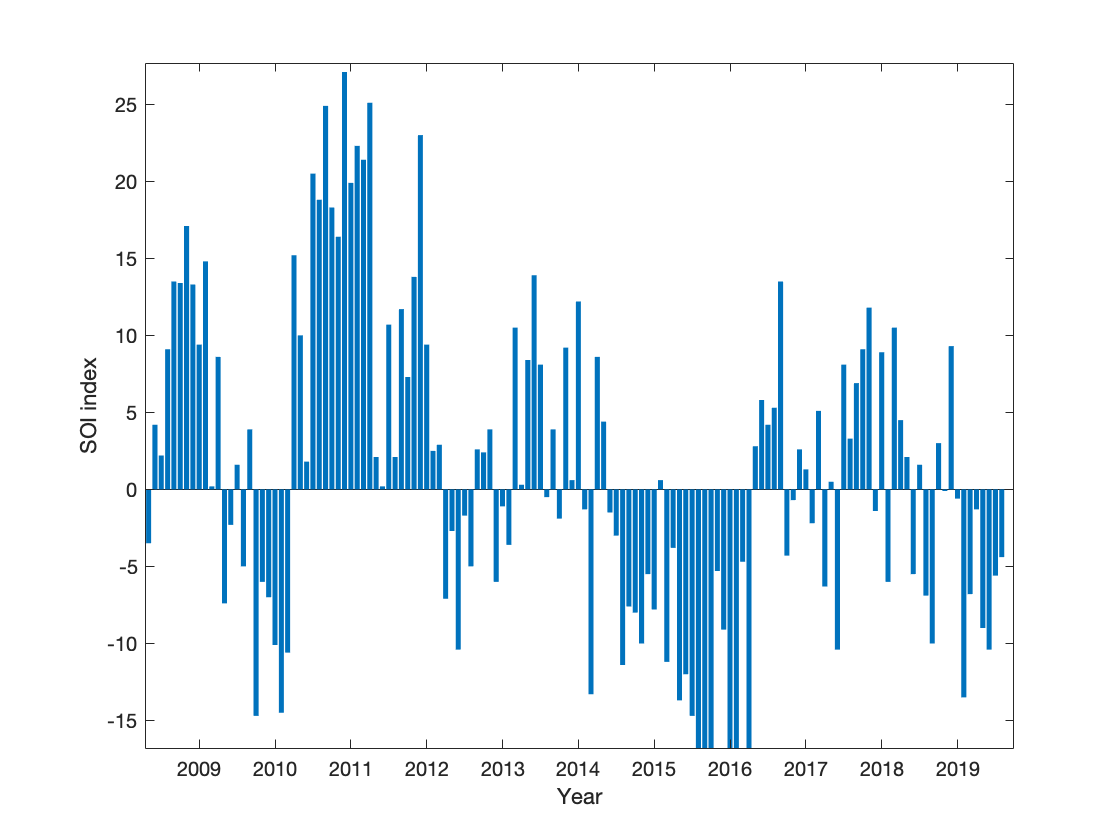
\includegraphics[width=0.75\linewidth]{./figures/soi_index_updated.png}
\end{centering}
\end{frame}

% %---------------------------------------------------------------------------

         
 \begin{frame}
   \frametitle{Can we quantify how much ENSO is affecting linear rates in SST and CF?}
   \framesubtitle{How different would the rates be if the extreme enso periods were removed}
   \vspace{-0.15in}
   \begin{itemize}
   \item Consider the linear SST rate from the NOAA Extended Reconstructed SST V5 - 60 years    
   \item Time period for the rate calculation is 1950-2010 
   \end{itemize}
   \vspace{0.1in}
   \centering
 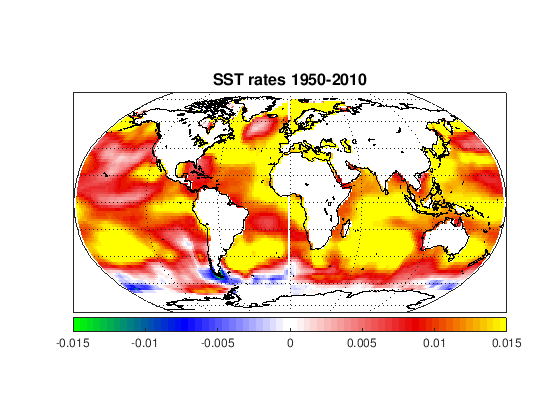
\includegraphics[width=0.4\linewidth]{./figures/sst_rates_1950_2010.png}
 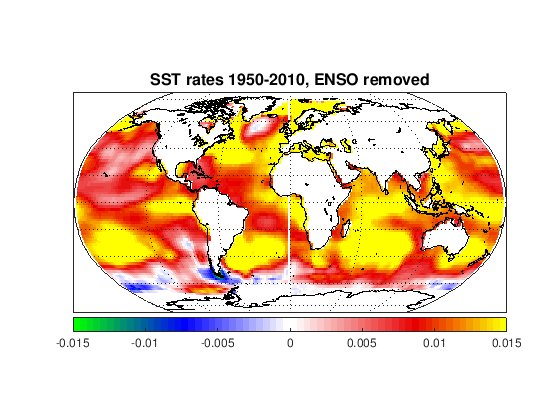
\includegraphics[width=0.4\linewidth]{./figures/sst_rates_1950_2010_enso_removed.png} \\ 
 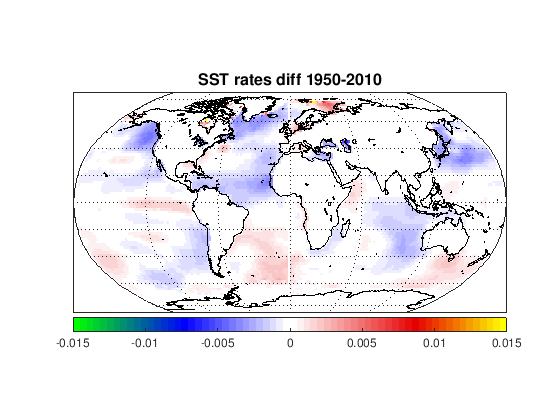
\includegraphics[width=0.4\linewidth]{./figures/sst_rates_diff_1950_2010.png} 
 \end{frame}
% %---------------------------------------------------------------------
% %---------------------------------------------------------------------
 \begin{frame}
  \frametitle{Impact of ENSO on 40 year SST rates}
 \begin{itemize}
    \item Impact of of ENSO is noticeably larger.   
%    \item PDF rate shows how occurences of a particular BT range are changing per year.
%    \item Color bar scale shows whether BT is increasing. 
%    \item Gray lines are where rate < uncertainty 
     \centering
    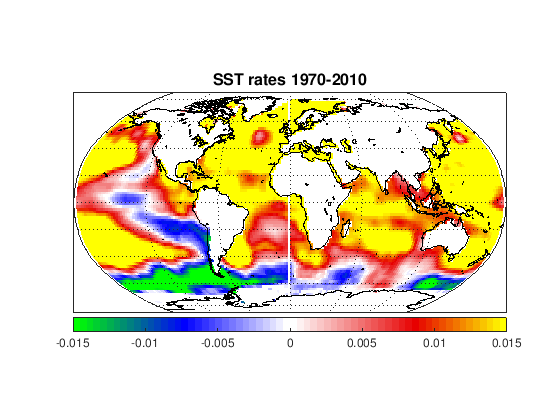
\includegraphics[width=0.4\linewidth]{./figures/sst_rates_1970_2010.png}
    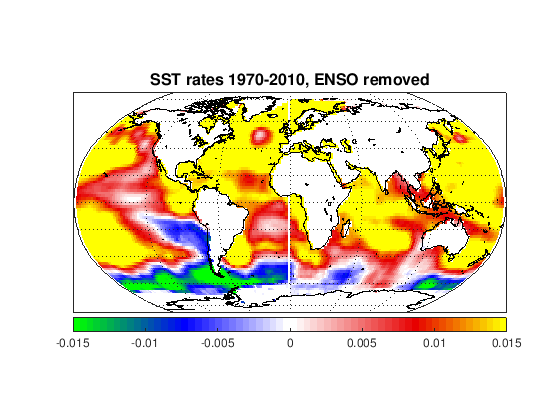
\includegraphics[width=0.4\linewidth]{./figures/sst_rates_1970_2010_enso_removed} \\
    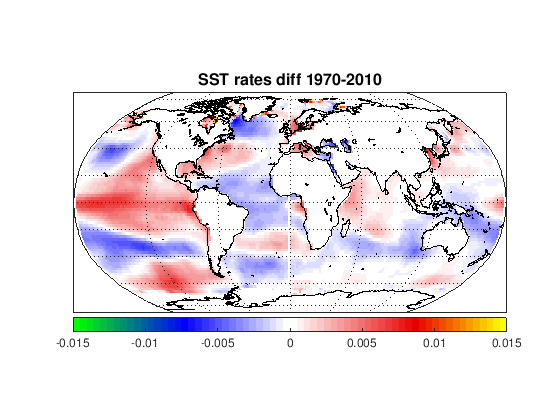
\includegraphics[width=0.4\linewidth]{./figures/sst_rates_diff_1970_2010} 
 \end{itemize}
 \end{frame}
% %---------------------------------------------------------------------
 \begin{frame}
  \frametitle{Impact of ENSO on 20 year SST rates}
 \begin{itemize}
    \item Maximum difference off the west coast of S. America. 
%    \item Clear Calculated Bt - Obs using ERA.
%    \item Averaged on 1x0.5 degree grid. 
 \end{itemize}
    \centering
    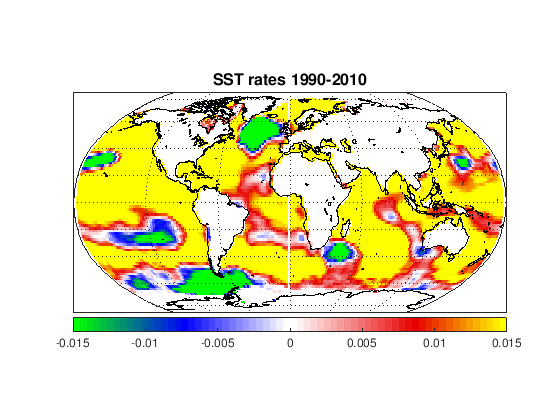
\includegraphics[width=0.4\linewidth]{./figures/sst_rates_1990_2010.png}
    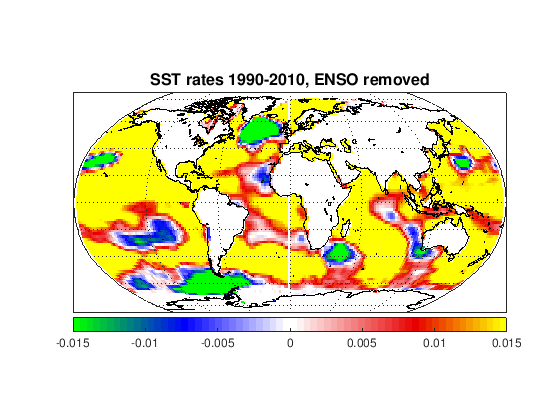
\includegraphics[width=0.4\linewidth]{./figures/sst_rates_1990_2010_enso_removed.png} \\ 
    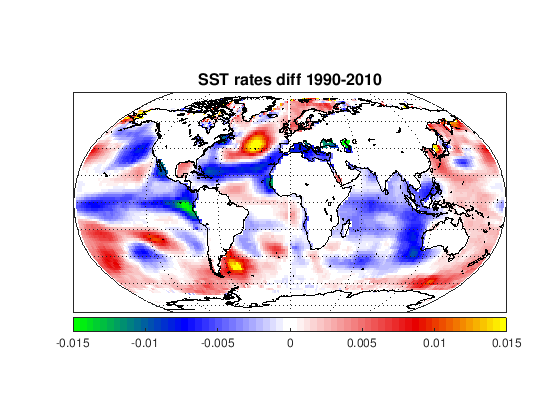
\includegraphics[width=0.4\linewidth]{./sst_rates_diff_1990_2010.png}  
 \end{frame}
% %---------------------------------------------------------------------
 \begin{frame}
  \frametitle{Relative RMS difference vs. number of years}
 \begin{itemize}
 \item Global differences depend on how many El Nino/La Nina events are included. 
 \item 16 year rates have a 10\% impact of ENSO.  
%   \item 1\% of data over 13 years.
 \end{itemize}
% \twocol{.55}{.55}
% {
\centering 
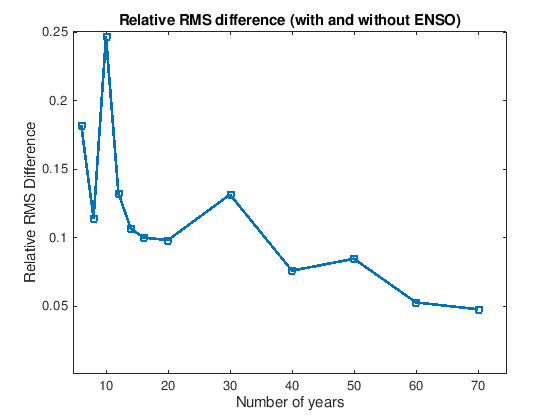
\includegraphics[width=0.7\linewidth]{./figures/RMS_rel_diff.png}
% }
% {
% \begin{block}{\tiny 5-15 K}
% %\includegraphics[width=\linewidth]{./Figs/map_mean_forcing_5to15K.png}
% \end{block}
% }
 \end{frame}
% %---------------------------------------------------------------------
 \begin{frame}
  \frametitle{Cloud Forcing: Surface Temperature - BT for WN $917.3 cm^{-1}$  }
 \begin{itemize}
    \item Mean CF in 2016 and 2018.
    \item Is there a signature of ENSO in the change of CF? 

 \end{itemize} 
%    \item 1\% of data over 13 years.
% \twocol{.55}{.55}
% {
% \begin{block}{\tiny 15-30 K }
\centering
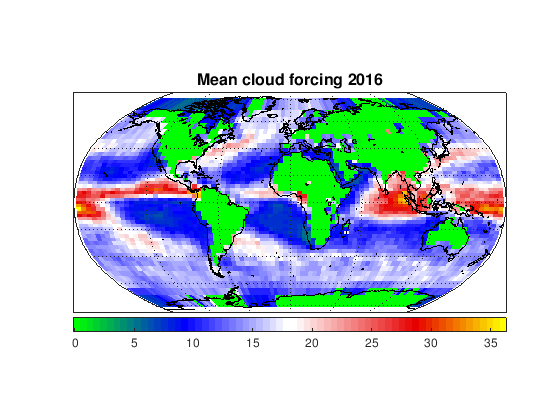
\includegraphics[width=.4\linewidth]{./figures/mean_cloud_forcing_2016.png}
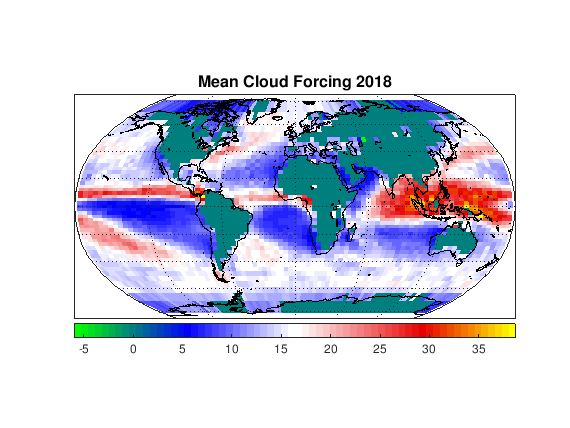
\includegraphics[width=.4\linewidth]{./figures/mean_cloud_forcing_2018.png} \\
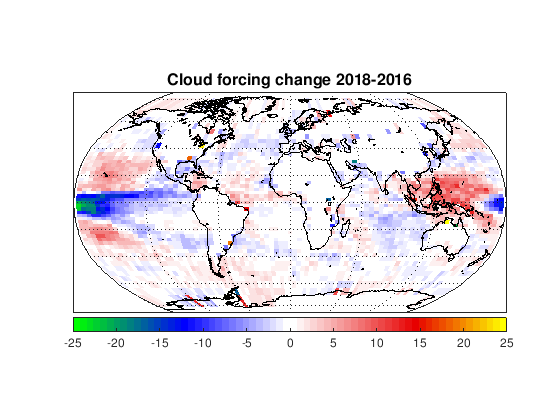
\includegraphics[width=.4\linewidth]{./figures/cloud_forcing_change_2016_2018.png} 
% \end{block}
% }
% {
% \begin{block}{\tiny 30-45 K}

% %\includegraphics[width=\linewidth]{./Figs/map_mean_forcing_30to45K.png}
% \end{block}
% }
 \end{frame}

% %---------------------------------------------------------------------
 \begin{frame}
  \frametitle{EOFs of CF}
% \begin{itemize} 
%   \item Color bar indicates PDF value.
%   \item Large values indicate deep convective clouds. 
%   \item Values near zero indicate clear sky.  
% \end{itemize} 
   \centering
   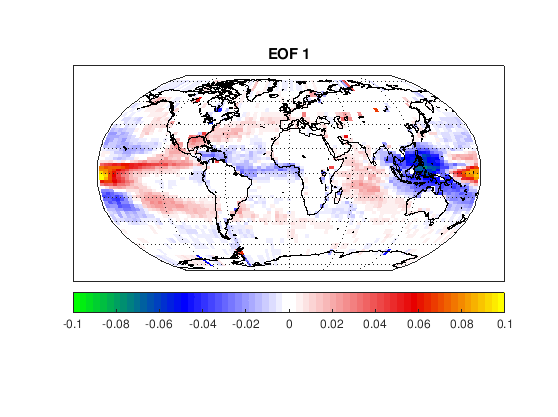
\includegraphics[width=0.4\linewidth]{./figures/eof_1.png}
   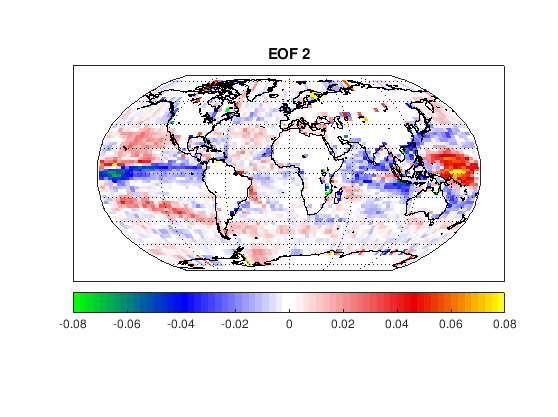
\includegraphics[width=0.4\linewidth]{./figures/eof_2.png} \\  
\begin{itemize} 
  \item EOF coefficients in time. First 2 peak in 2016. 
  \item Can we use EOFs to get a handle on how much ENSO is impacting CF? 
   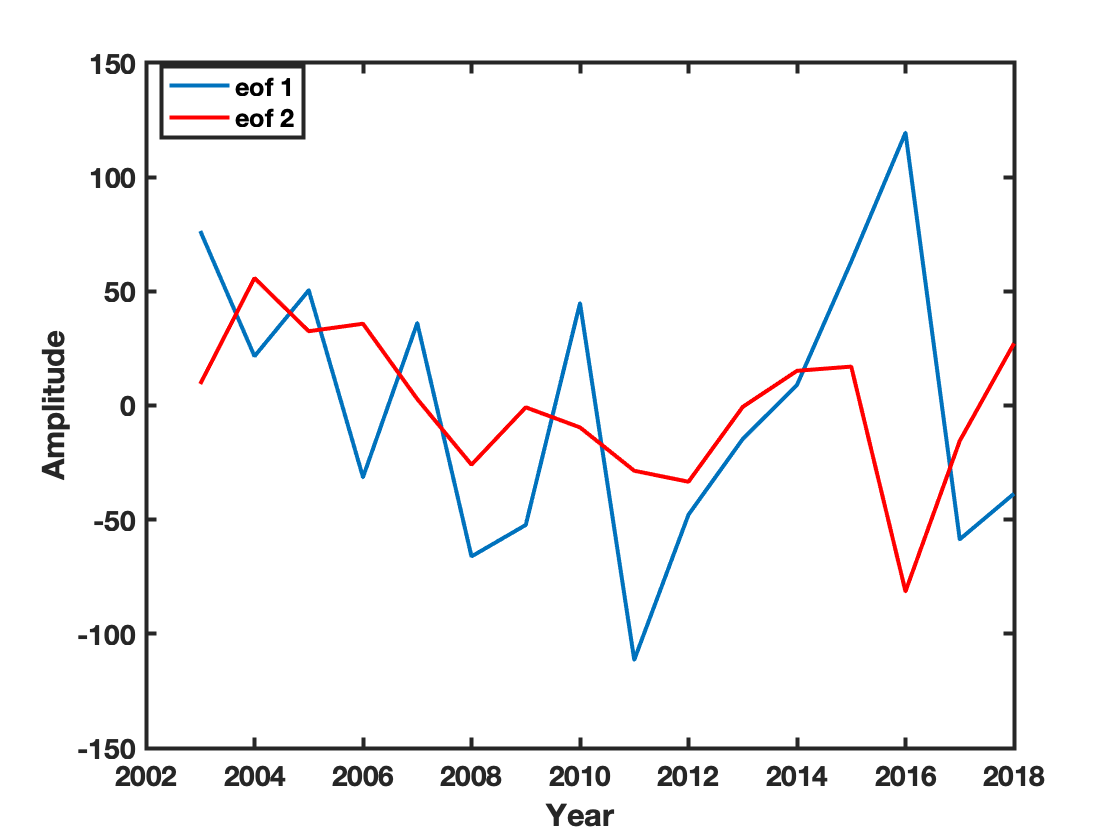
\includegraphics[width=0.4\linewidth]{./figures/eofs_1_2.png}  
\end{itemize} 
 \end{frame}

\begin{frame}[label={sec:org273b7f2}]{Cloud Forcing Global Behavior}
\begin{itemize}
\item Something for which AIRS may have a unique contribution
\item Define CF = SST - BTobs.  (more cloud means positive)
\item Global: maybe interesting, what does AIRS stability tell us?
\item ENSO:  how does cloud forcing respond to an ENSO kick?
\item We know SST very well, we know BTobs very well.
\item Of course, global dominated by tropics
\end{itemize}
\end{frame}

\begin{frame}[label={sec:org0ddce1e}]{Global SST and BTobs Anomalies}
\begin{center}
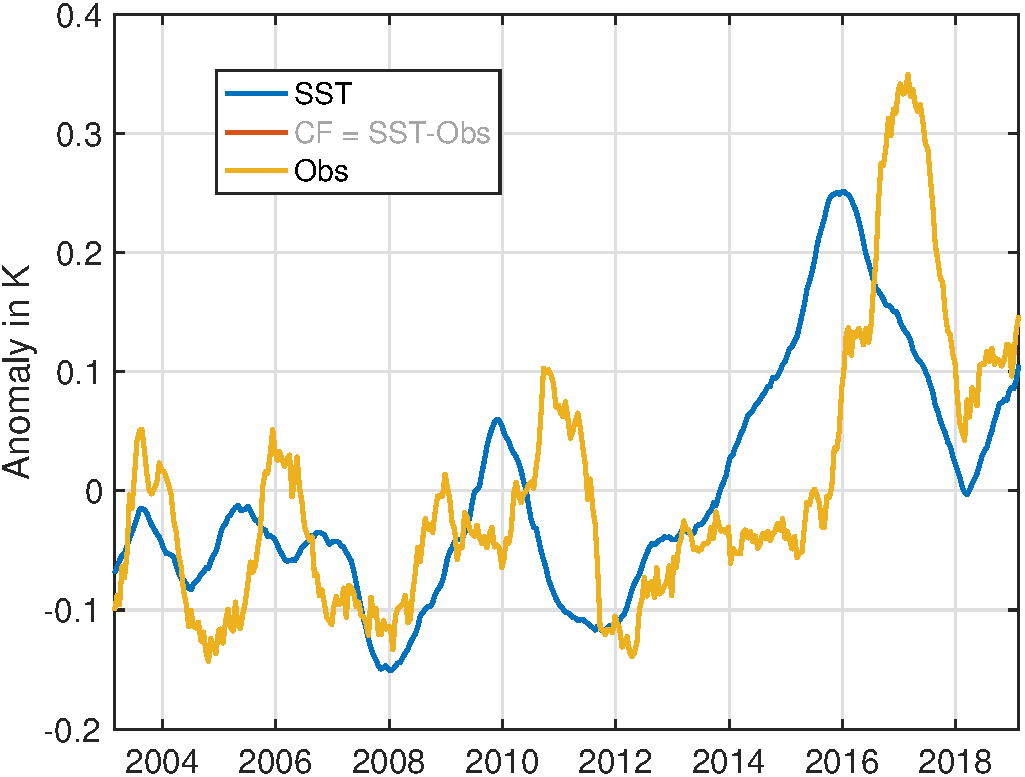
\includegraphics[width=0.7\linewidth]{./Figs/Pdf/tseries_sst_obs_global.pdf}
\end{center}
\end{frame}


\begin{frame}[label={sec:org4293227}]{Now Add Longwave Cloud Forcing}
\begin{center}
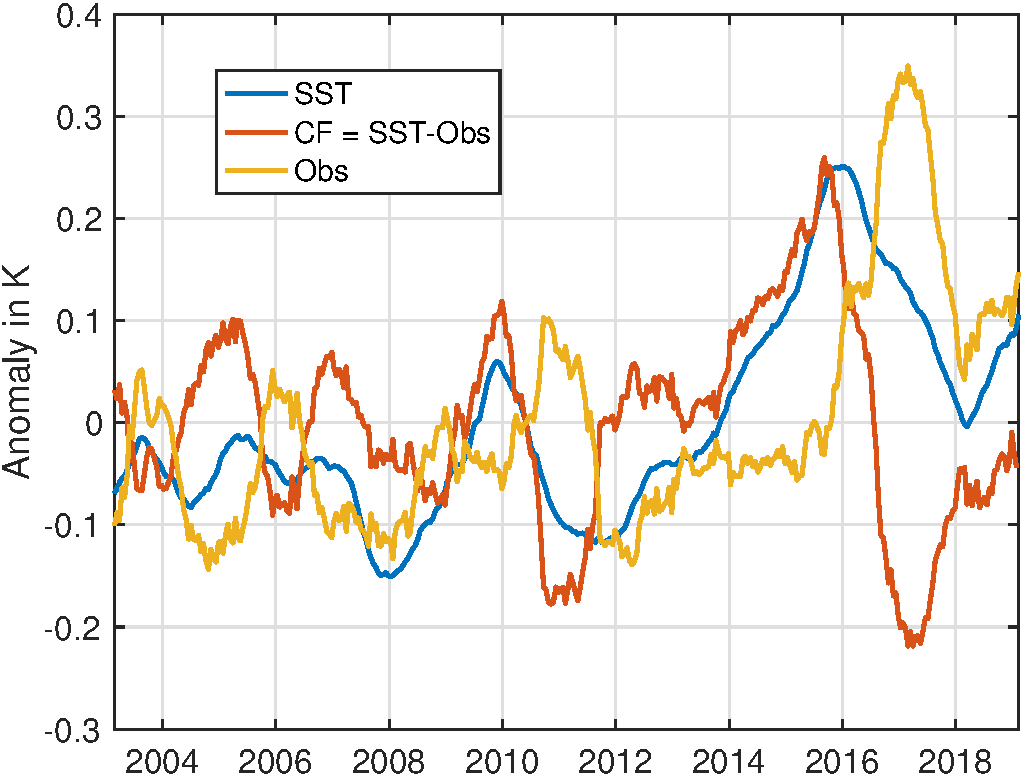
\includegraphics[width=0.7\linewidth]{./Figs/Pdf/tseries_sst_cf_obs_global.pdf}
\end{center}

\small 
\begin{itemize}
\item Note sharp CF drop at SST peak anomaly
\end{itemize}
\end{frame}

\begin{frame}[label={sec:org313609b}]{Delay of BTobs Anomaly to SST Anomaly}
\begin{center}
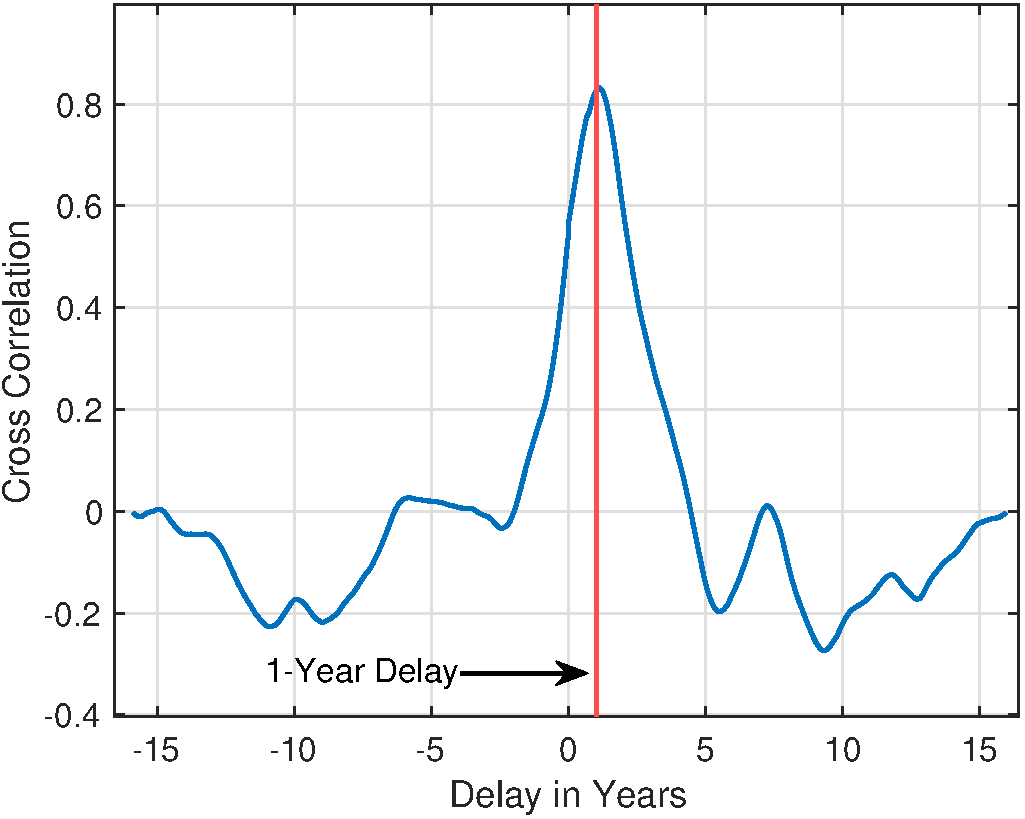
\includegraphics[width=0.7\linewidth]{./Figs/Pdf/ocean_btobs_delay_from_sst.pdf}
\end{center}

\small 
\begin{itemize}
\item Almost exactly a 1-year delay in BTobs (clear trend) from SST
\end{itemize}
\end{frame}

\begin{frame}[label={sec:org16736e3}]{Examine Time Dependence of CF vs SST Anomaly}
\vspace{-0.15in}
\begin{center}
\includegraphics[width=0.7\linewidth]{./Figs/Png/cf_vs_sst_vs_year.png}
\end{center}

\vspace{-0.15in}
\footnotesize
\begin{itemize}
\item At peak of ENSO CF drops very quickly
\item Overshoots
\item Then back to normal, BUT, of course, SST has gone up by a tremendous amount in a short time: 0.15K
\end{itemize}
\end{frame}

\begin{frame}[label={sec:org6f50560}]{CF vs ENSO Index}
\begin{center}
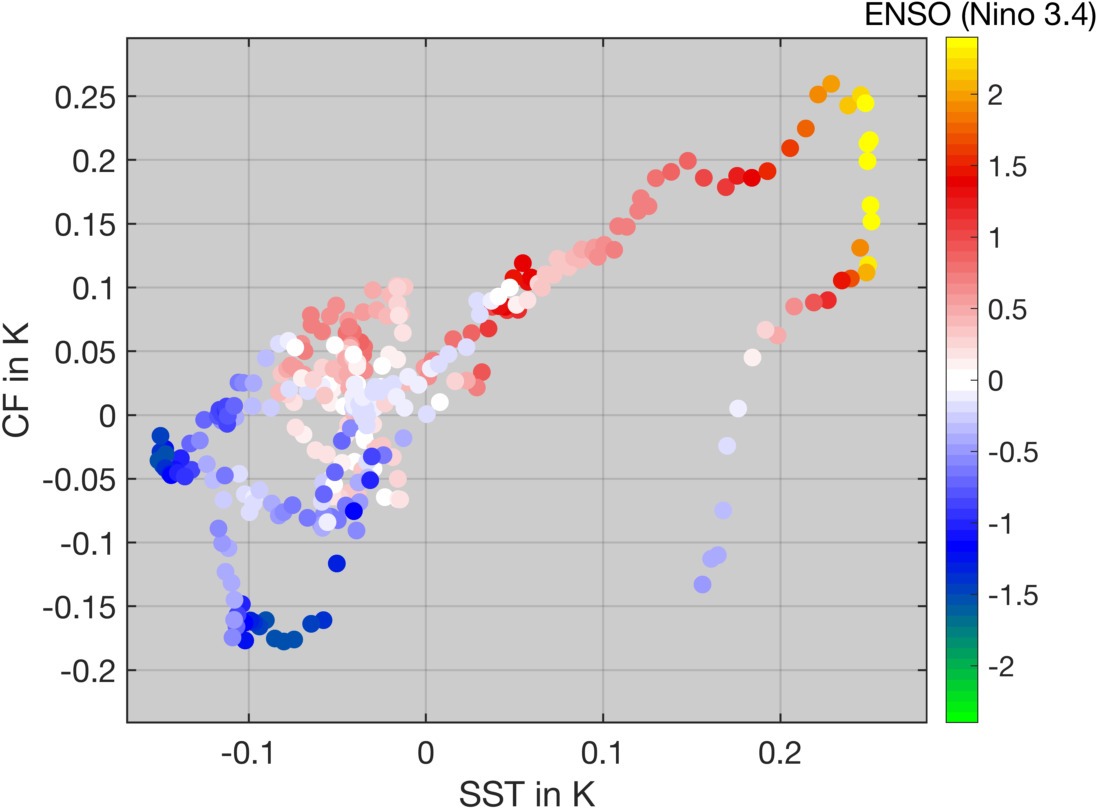
\includegraphics[width=0.7\linewidth]{./Figs/Png/cf_vs_sst_vs_enso_v2.png}
\end{center}

\footnotesize
\begin{itemize}
\item ENSO returns to normal, CF returns
\end{itemize}
\end{frame}

\begin{frame}[label={sec:orgd9a47e3}]{Climate Model Cloud Trends (Trenberth, 2009)}
\begin{center}
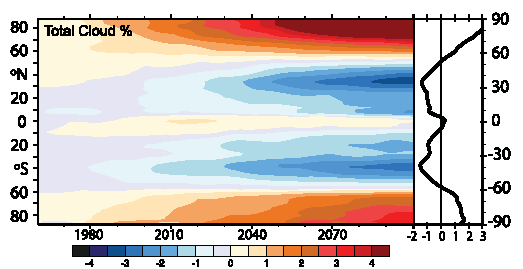
\includegraphics[width=0.9\linewidth]{./Figsc/Pdf/trenberth2009_clouds_top.pdf}
\end{center}
\end{frame}

\begin{frame}{CF Trends: \small Left: Trenberth (2009) \%/150 years,   Right: AIRS}.

\vspace{-0.1in}
  % \begin{columns}
% \begin{column}{0.55\columnwidth}
% \begin{block}{Climate Model Cfraction Trend}
% \begin{center}
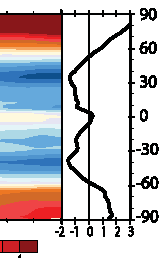
\includegraphics[width=0.34\linewidth]{./Figsc/Pdf/trenberth_total_only.pdf}
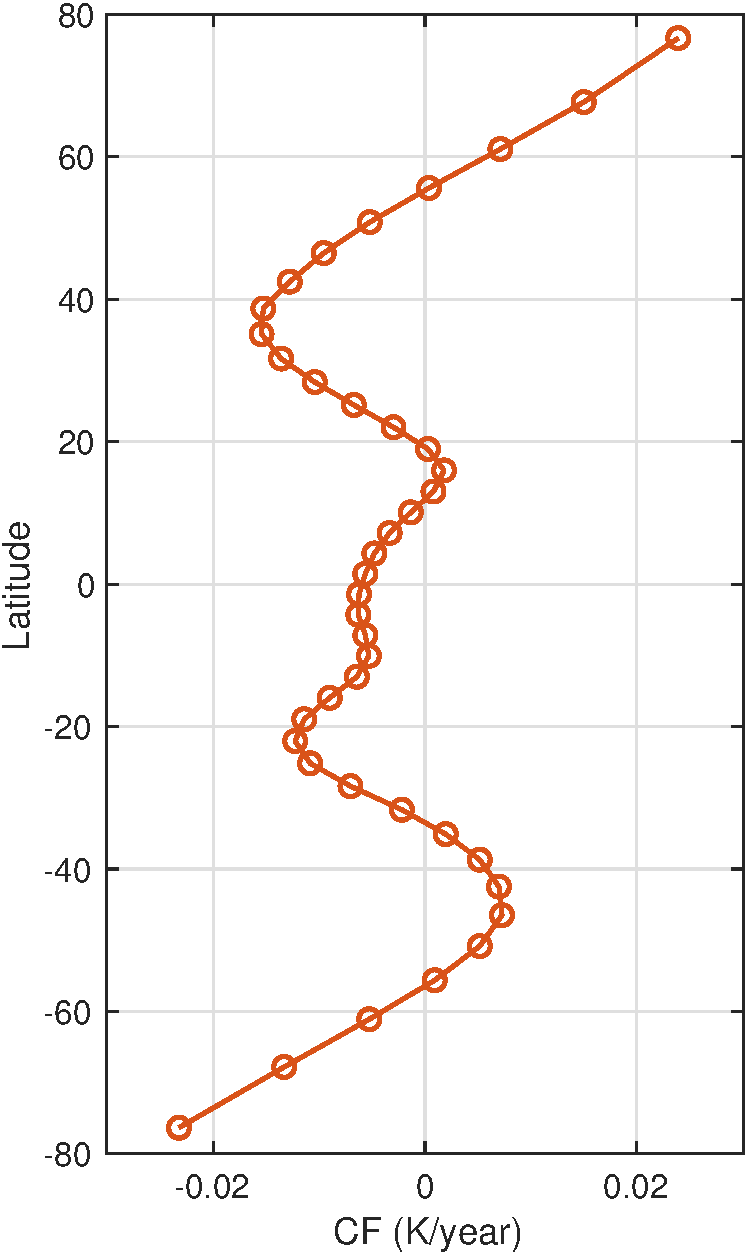
\includegraphics[width=0.3\linewidth]{./Figsc/Pdf/new_trend_rand_stats_1231_and_2161_era_clr_minus_obs_smoothed.pdf}
% \end{center}
% \end{block}
% \end{column}

\vspace{-0.1in}

\begin{footnotesize}
  \begin{itemize}
    \item  AIRS cloud forcing fractional change $\sim$5X higher than models
\item  Clearly we may just be observing fragments from ENSO, need time
\item But, climate model uncertainty large
\item  AIRS stability likely 3x better than obs
\item  Need stable surface T also, derive using AIRS for consistency
\end{itemize}
\end{footnotesize}


% \begin{column}{0.55\columnwidth}
% \begin{block}{AIRS CF Trend}
% \begin{center}
%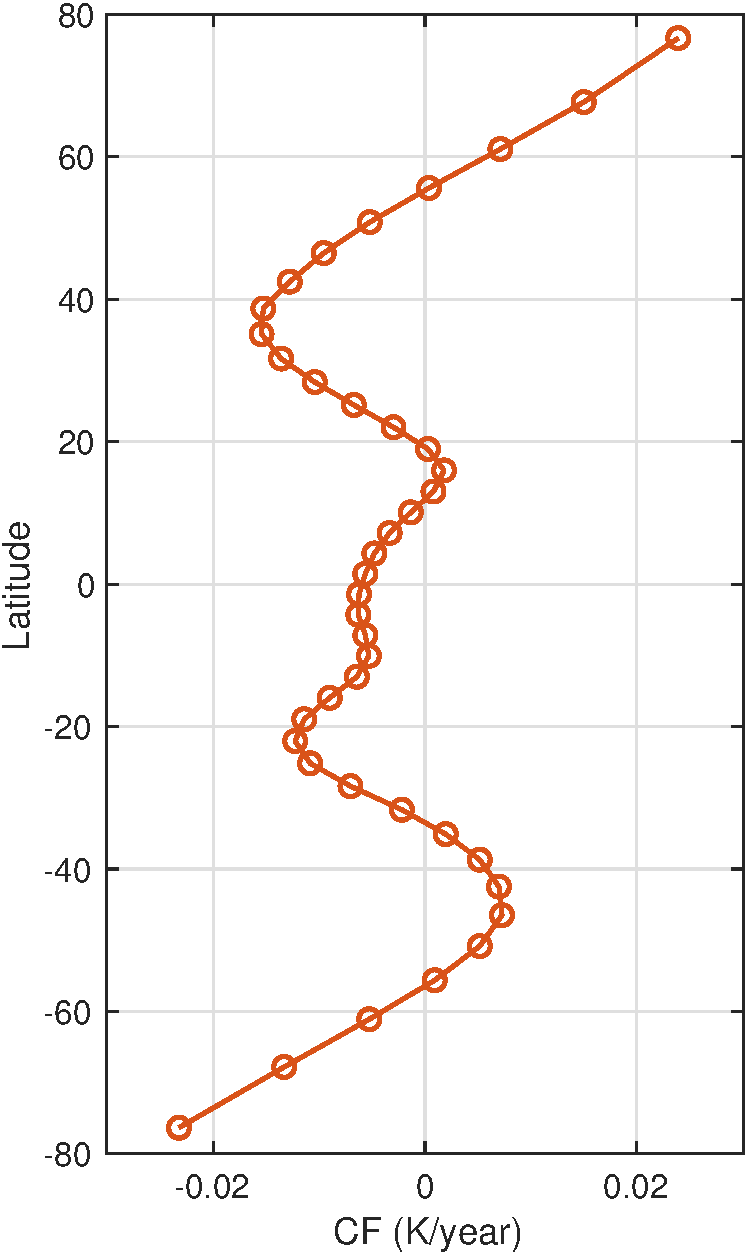
\includegraphics[width=0.3\linewidth]{./Figsc/Pdf/new_trend_rand_stats_1231_and_2161_era_clr_minus_obs_smoothed.pdf}
% \end{center}
% \end{block}
% \end{column}
% \end{columns}
\end{frame}


\begin{frame}[label={sec:org16736e3}]{AIRS Connection with Shortwave Cloud Forcing}
\vspace{-0.15in}
\begin{center}
  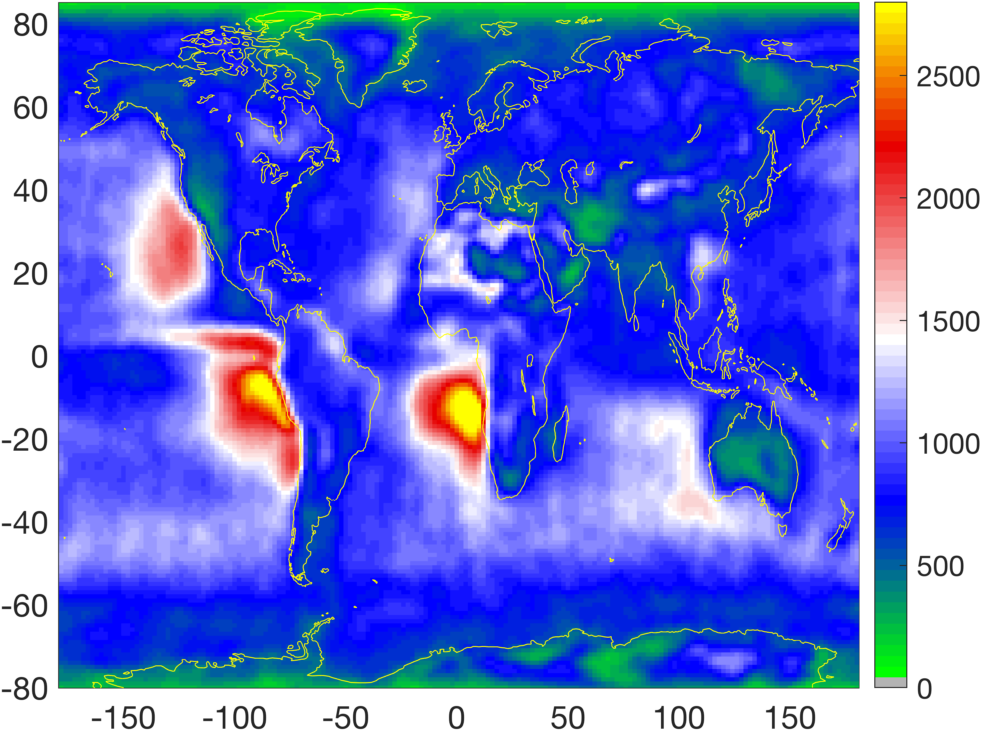
\includegraphics[width=0.65\linewidth]{./map_mbl_4K_to_10K_with_land.png}
\end{center}
\vspace{-0.15in}
\footnotesize
\begin{itemize}
\item With a good surface T, marine boundary layer (MBL) clouds easy to detect (BTobs 4-10K lower than surface T)
\item They represent one of the largest contributors to cloud radiative effect in climate models increasing MBL clouds greatly affect reflected solar with little change to longwave forcing
\item We can very precisely monitor changes in MBL clouds using BTsurface - BTobs
\end{itemize}
\end{frame}



\end{document}

